\subsubsection{$d_{AB}(t)$ from $\frac{t}{T} \in \left[ 998, 1000\right]$}
%%%%%%%%%%%%%%%%%%%%%%%%%%%%%%%%%%%%%%%%%%%%%%%%%%%%
%  				    FIGURE 					       %
%%%%%%%%%%%%%%%%%%%%%%%%%%%%%%%%%%%%%%%%%%%%%%%%%%%%
% TOLERANCE 1 * 10^{-7}
% 998-1,000 t/T
\begin{figure}[h]
	\begin{subfigure}[b]{0.5\textwidth}
		{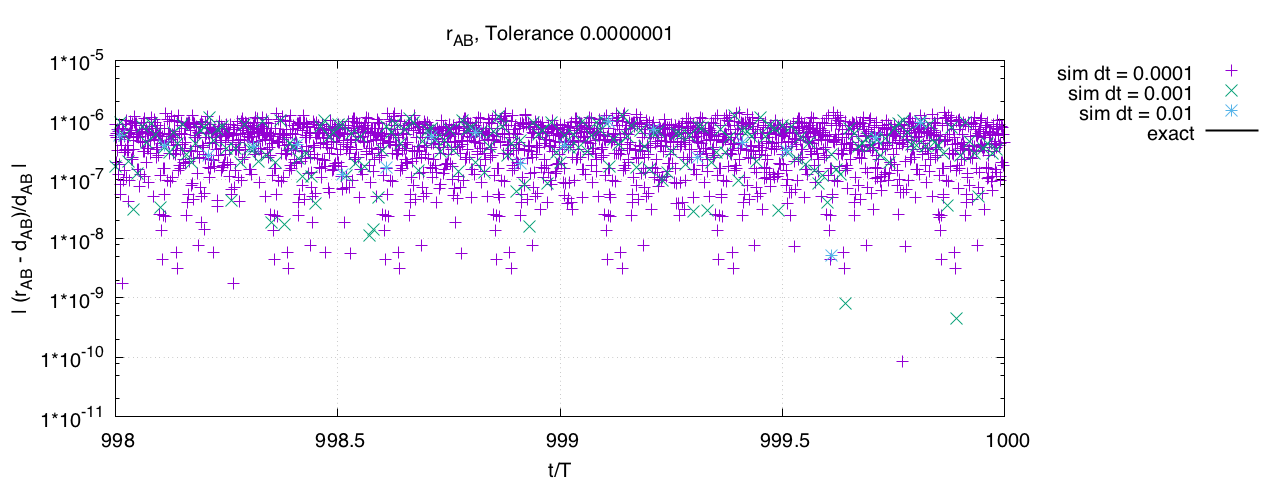
\includegraphics[width=\textwidth]
			{tol_0p0000001_dab_vs_sampleTime_endtime_0p1.png}}
		\caption{tolerance $1 \times 10^{-7}$, $\frac{t}{T}$ from $998$ to $1000$}
	\end{subfigure}
	\vfill
	% TOLERANCE 1 * 10^{-5}
	% 8-10 t/T
	\begin{subfigure}[b]{0.5\textwidth}
		{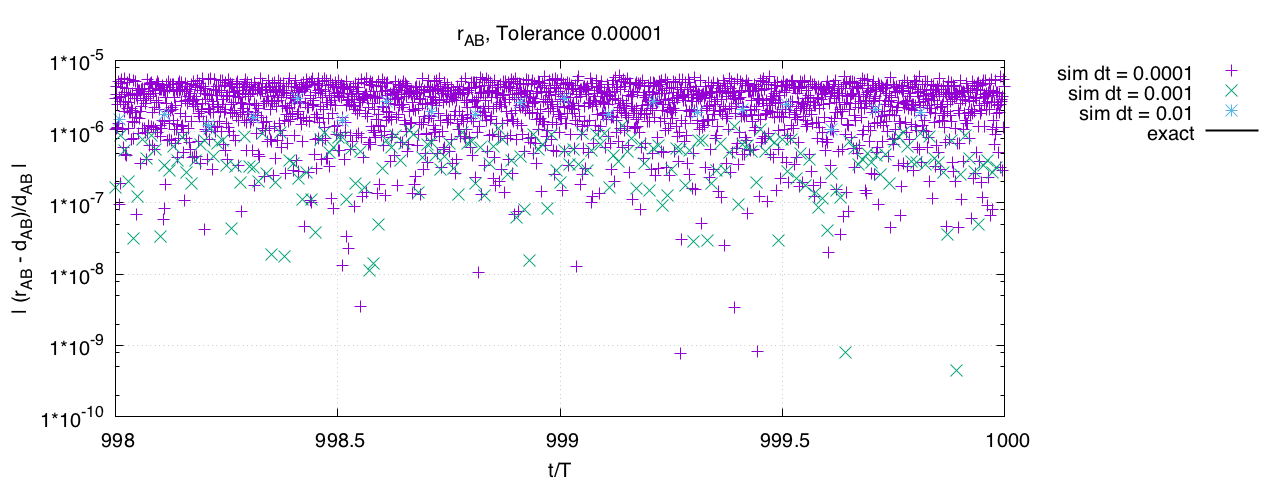
\includegraphics[width=\textwidth]
			{tol_0p00001_dab_vs_sampleTime_endtime_0p1.png}}
		\caption{tolerance $1 \times 10^{-5}$, $\frac{t}{T}$ from $998$ to $1000$}
	\end{subfigure}
	\vfill
	% TOLERANCE 1 * 10^{-3}
	% 8-10 t/T
	\begin{subfigure}[b]{0.5\textwidth}
		{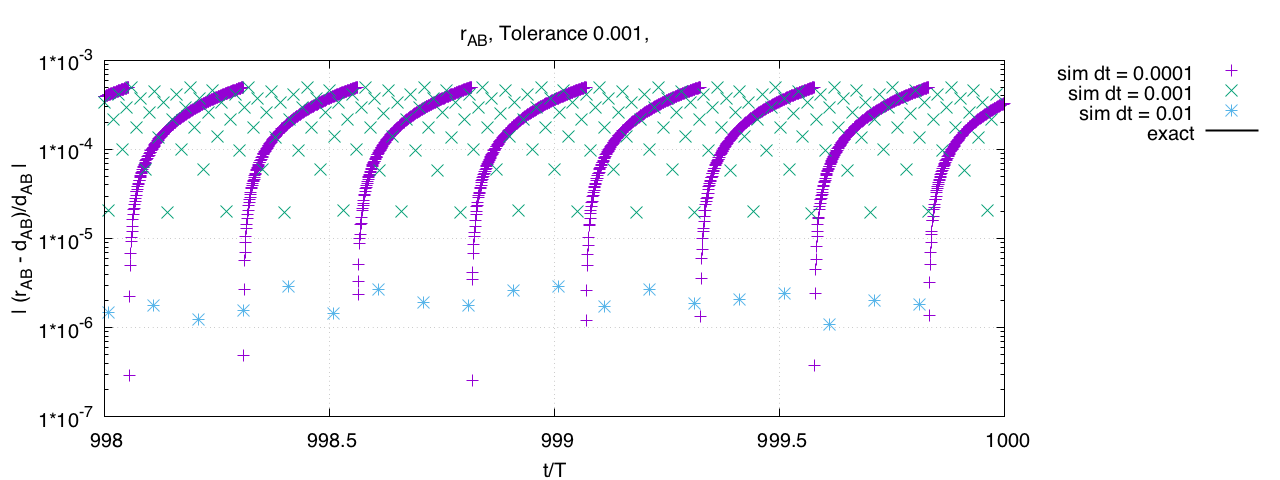
\includegraphics[width=\textwidth]
			{tol_0p001_dab_vs_sampleTime_endtime_0p1.png}}
		\caption{tolerance $1 \times 10^{-3}$, $\frac{t}{T}$ from $998$ to $1000$}
	\end{subfigure}
	\vfill
	% TOLERANCE 1 * 10^{-1}
	% 9,998-10,000 t/T
	\begin{subfigure}[b]{0.5\textwidth}
		{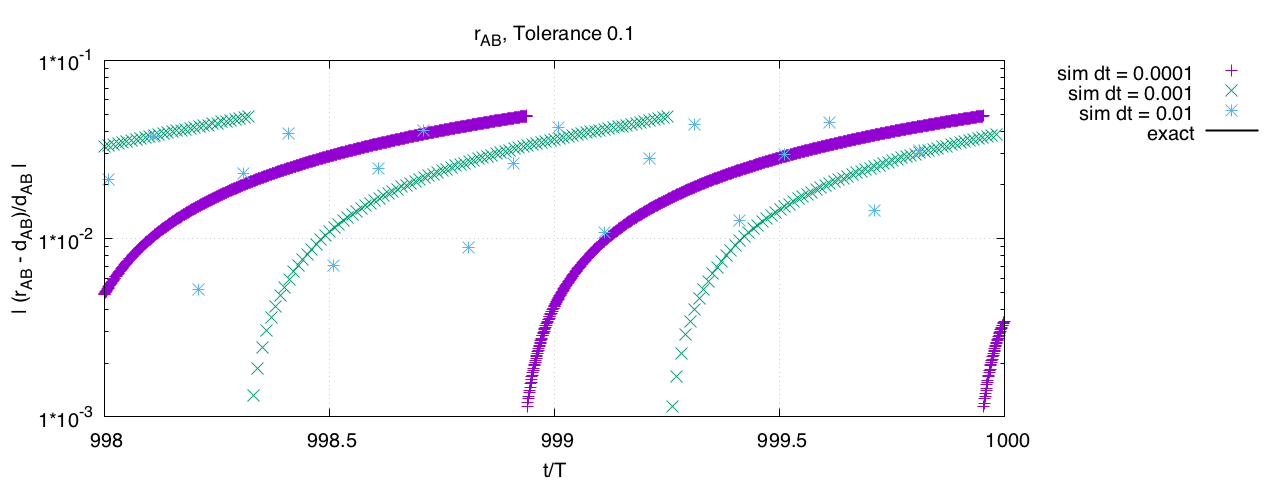
\includegraphics[width=\textwidth]
			{tol_0p1_dab_vs_sampleTime_endtime_0p1.png}}
		\caption{tolerance $1 \times 10^{-1}$, $\frac{t}{T}$ from $998$ to $1000$}
	\end{subfigure}
	\caption{\label{fig:res-dab-1} The bond length in the diatomic molecule, at various tolerance levels and at $\frac{t}{T} \in \left[ 9998, 10000 \right]$ during the simulation. The two different tolerances in the $\textsf{RATTLE}$ algorithm were set equal.}
\end{figure}
%%%%%%%%%%%%%%%%%%%%%%%%%%%%%%%%%%%%%%%%%%%%%%%%%%%%